\documentclass[11pt,a4paper]{article}
\usepackage[utf8]{inputenc}
\usepackage[vietnamese]{babel}
\usepackage{amsmath,amssymb}
\usepackage[version=4]{mhchem}
\usepackage{geometry}
\geometry{top=0.65cm,bottom=0.65cm,left=1.25cm,right=1.25cm,headheight=20pt,headsep=3pt,footskip=9pt}
\usepackage{graphicx}
\usepackage{xcolor}
\usepackage{tabularx}
\usepackage{array}
\usepackage{tikz}
\usepackage{multicol}
\usepackage{fancyhdr}
\usepackage{enumitem}

\definecolor{hfRed}{HTML}{D32F2F}
\definecolor{hfGreen}{HTML}{8BC390}
\definecolor{mainGreen}{HTML}{2E7D32}

\usepackage{ex_test}

\pagestyle{fancy}
\fancyhf{}
\renewcommand{\headrulewidth}{0.75pt}
\renewcommand{\headrule}{\hbox to\headwidth{\color{hfGreen}\leaders\hrule height \headrulewidth\hfill}}
\renewcommand{\footrulewidth}{0.75pt}
\renewcommand{\footrule}{\hbox to\headwidth{\color{hfGreen}\leaders\hrule height \footrulewidth\hfill}}

\fancyhead[L]{\small\itshape\color{hfRed}Tài liệu lưu hành nội bộ}
\fancyhead[R]{\small\color{hfRed}Thầy \textbf{TRẦN VĂN THẠNH} - 0777.470.803}

\fancyfoot[L]{\footnotesize\itshape\color{hfRed}CS1: 6/15 Nguyễn Hoàng, P. Kim Long, TP Huế \quad|\quad CS2: 24 Đặng Thái Thân, TP Huế}
\fancyfoot[R]{\small\textbf{\color{hfRed}Trang \thepage}}

\setlength{\parindent}{0pt}
\setlength{\parskip}{0.0pt}

\def\loigiai#1{}

\begin{document}
\Opensolutionfile{ans}[ans-de19-hs]

\noindent
\begin{minipage}[t]{0.48\textwidth}
	\textbf{SỞ GIÁO DỤC VÀ ĐÀO TẠO THỪA THIÊN HUẾ}\\
	\textbf{TRƯỜNG THPT HAI BÀ TRƯNG}\\
	\textbf{ĐỀ CHÍNH THỨC}\\
	\textit{(Đề thi có 04 trang)}
\end{minipage}\hfill
\begin{minipage}[t]{0.48\textwidth}
	\raggedleft
	\textbf{\color{mainGreen}ĐỀ KIỂM TRA ĐỊNH KỲ CHƯƠNG 7 (KIM LOẠI NHÓM IA \& IIA)}\\
	\textbf{MÔN: HOÁ HỌC -- LỚP 12}\\
	\textit{Thời gian làm bài: 50 phút (không kể thời gian phát đề)}\\
	\textbf{Mã đề thi: 119}
\end{minipage}


\vspace{1pt}
\noindent\textit{Họ, tên thí sinh: \dots\dots\dots\dots\dots\dots\dots\dots\dots\dots\dots\dots\dots\dots\dots\dots\dots\dots\dots\dots\dots\dots Lớp: \dots\dots\dots\dots SBD: \dots\dots\dots\dots}\\
\noindent\textit{(Cho biết nguyên tử khối: H = 1; C = 12; N = 14; O = 16; Na = 23; Mg = 24; Al = 27; P = 31; S = 32; Cl = 35,5; K = 39; Ca = 40; Fe = 56; Cu = 64; Zn = 65; Br = 80; Rb = 85,5; Ag = 108; Cs = 133; Ba = 137).}

\vspace{1pt}
\noindent
\textbf{PHẦN I (4,5 điểm -- 18 câu): Câu trắc nghiệm nhiều phương án lựa chọn.}\\
\textit{Thí sinh trả lời từ câu 1 đến câu 18. Mỗi câu hỏi thí sinh chỉ chọn một phương án.}

\begin{ex}
Các đại dương là những kho muối vô tận với nhiều khoáng chất có giá trị dinh dưỡng cao. Trong nước biển, hai nguyên tố kim loại có nhiều nhất là
\choice
{sodium và magnesium.}
{đồng (copper) và kẽm (zinc).}
{nhôm (aluminium) và sắt (iron).}
{vàng (gold) và bạc (silver).}
\loigiai{}
\end{ex}

\begin{ex}
Cấu hình electron lớp ngoài cùng của nguyên tử kim loại kiềm là
\choice
{$ns^2np^2$.}
{$ns^2np^1$.}
{$ns^1$.}
{$ns^2$.}
\loigiai{}
\end{ex}

\begin{ex}
Kim loại nào sau đây là kim loại kiềm?
\choice
{Na.}
{Ca.}
{Al.}
{Fe.}
\loigiai{}
\end{ex}

\begin{ex}
Cho một mẩu Na vào dung dịch \ce{MgSO4} dư, thu được kết tủa X và chất khí Y. Hai chất X, Y lần lượt là
\choice
{Mg và \ce{H2}.}
{\ce{Mg(OH)2} và \ce{H2}.}
{Mg và \ce{O2}.}
{\ce{Na2SO4} và \ce{H2}.}
\loigiai{}
\end{ex}

\begin{ex}
Trong cốc nước chứa nhiều các ion sau: \ce{Ca^2+}, \ce{Mg^2+}, \ce{Cl-}, \ce{SO4^2-}. Nước trong cốc trên thuộc loại
\choice
{có tính cứng vĩnh cửu.}
{không có tính cứng.}
{có tính cứng tạm thời.}
{có tính cứng toàn phần.}
\loigiai{}
\end{ex}

\begin{ex}
Nhận định nào \textbf{không} đúng về cấu tạo và tính chất của các kim loại nhóm IIA?
\choice
{Khối lượng riêng tương đối nhỏ, là những kim loại nhẹ hơn nhôm (trừ Ba).}
{Độ cứng cao hơn kim loại nhóm IA, nhưng mềm hơn kim loại nhôm.}
{Mạng tinh thể của chúng đều có kiểu lập phương tâm khối.}
{Nhiệt độ nóng chảy và nhiệt độ sôi tương đối thấp (trừ Be).}
\loigiai{}
\end{ex}

\begin{ex}
Phương trình hóa học của phản ứng nào sau đây \textbf{không} đúng?
\choice
{$\ce{Ca + 2H2O -> Ca(OH)2 + H2}$.}
{$\ce{BeO + H2O -> Be(OH)2}$.}
{$\ce{Mg + H2SO4 -> MgSO4 + H2}$.}
{$\ce{Be + 2NaOH -> Na2BeO2 + H2}$.}
\loigiai{}
\end{ex}

\begin{ex}
Cách nào sau đây \textbf{không} thu được NaOH sau phản ứng?
\choice
{Điện phân dung dịch \ce{NaCl} không có màng ngăn xốp.}
{Cho kim loại Na tác dụng với nước.}
{Điện phân dung dịch \ce{NaCl} có màng ngăn xốp, điện cực trơ.}
{Cho dung dịch \ce{Ca(OH)2} tác dụng với dung dịch \ce{Na2CO3}.}
\loigiai{}
\end{ex}

\begin{ex}
Hai chất nào sau đây được dùng để làm mềm nước có tính cứng vĩnh cửu?
\choice
{\ce{NaCl} và \ce{Ca(OH)2}.}
{\ce{Na2CO3} và \ce{Na3PO4}.}
{\ce{Na2CO3} và \ce{Ca(OH)2}.}
{\ce{Na2CO3} và \ce{HCl}.}
\loigiai{}
\end{ex}

\newpage

\begin{ex}
Hợp chất Y của calcium là thành phần chính của vỏ các loại ốc, sò,... Ngoài ra Y được sử dụng rộng rãi trong sản xuất vôi, xi măng, thuỷ tinh, chất phụ gia trong công nghiệp thực phẩm. Hợp chất Y là
\choice
{\ce{CaO}.}
{\ce{CaCO3}.}
{\ce{Ca(OH)2}.}
{\ce{Ca3(PO4)2}.}
\loigiai{}
\end{ex}

\begin{ex}
Kim loại \textbf{không} phản ứng với nước ở nhiệt độ thường là
\choice
{Be.}
{Ca.}
{Li.}
{K.}
\loigiai{}
\end{ex}

\begin{ex}
Xét phản ứng phân huỷ muối carbonate của kim loại nhóm IIA: $\ce{MCO3(s) -> MO(s) + CO2(g)} \quad (\Delta_r H^\circ_{298})$.\\
Từ \ce{MgCO3} đến \ce{BaCO3}, biến thiên enthalpy chuẩn của phản ứng biến đổi như thế nào?
\choice
{Không đổi.}
{Giảm dần.}
{Tăng dần.}
{Không có quy luật.}
\loigiai{}
\end{ex}

\begin{ex}
Ở nhiệt độ thường, độ tan của các hydroxide tăng dần trong dãy từ \ce{Mg(OH)2} đến \ce{Ba(OH)2}. Từ thông tin này có thể dự đoán được khả năng phản ứng với nước của các kim loại từ Mg đến Ba biến đổi như thế nào?
\choice
{Tăng dần.}
{Không đổi.}
{Không có quy luật.}
{Giảm dần.}
\loigiai{}
\end{ex}

\begin{ex}
Nước chứa nhiều các ion nào sau đây có tính cứng toàn phần?
\choice
{\ce{Mg^2+}, \ce{Ca^2+}, \ce{HCO3-}, \ce{SO4^2-}, \ce{Cl-}.}
{\ce{Na+}, \ce{K+}, \ce{SO4^2-}, \ce{Cl-}.}
{\ce{Mg^2+}, \ce{Ca^2+}, \ce{HCO3-}.}
{\ce{Mg^2+}, \ce{Ca^2+}, \ce{SO4^2-}, \ce{Cl-}.}
\loigiai{}
\end{ex}

\begin{ex}
Phân tích một mẫu nước tự nhiên thấy chứa nhiều các ion: \ce{Na+}, \ce{Ca^2+}, \ce{HCO3-}, \ce{Cl-} và \ce{SO4^2-}. Chất nào sau đây có thể làm mềm mẫu nước trên?
\choice
{\ce{Na2CO3}.}
{\ce{Ca(OH)2}.}
{\ce{NaOH}.}
{\ce{HCl}.}
\loigiai{}
\end{ex}

\begin{ex}
Một loại nước cứng khi đun sôi thì trở thành nước mềm. Trong loại nước này có hoà tan những hợp chất nào sau đây?
\choice
{\ce{Ca(HCO3)2} và \ce{Mg(HCO3)2}.}
{\ce{Ca(HCO3)2} và \ce{MgSO4}.}
{\ce{CaSO4} và \ce{MgCl2}.}
{\ce{MgCl2} và \ce{CaCl2}.}
\loigiai{}
\end{ex}

\begin{ex}
Tiến hành thí nghiệm theo các bước sau:\\
\textbf{Bước 1:} Chuẩn bị hai ống nghiệm, ống (1) chứa 2 mL dung dịch \ce{CaCl2} 1 M, ống (2) chứa 2 mL dung dịch \ce{BaCl2} 1 M.\\
\textbf{Bước 2:} Nhỏ đồng thời vào mỗi ống nghiệm 3 giọt dung dịch \ce{CuSO4} 1 M, thấy ống (1) xuất hiện kết tủa chậm hơn và ít hơn so với ống (2).\\
Nhận định nào sau đây đúng khi so sánh \ce{CaSO4} với \ce{BaSO4}?
\choice
{Khó nhiệt phân hơn.}
{Khó thuỷ phân hơn.}
{Dễ kết tủa hơn.}
{Dễ tan hơn.}
\loigiai{}
\end{ex}

\begin{ex}
Cho sơ đồ chuyển hoá sau:\\
$\ce{CaO} \xrightarrow{+\text{X}} \text{Y} \xrightarrow{+\text{Z}} \ce{CaCO3} \xrightarrow{+\text{Z} + \text{X}} \text{T} \xrightarrow{+\text{E}} \ce{CaSO4}$\\
Biết: X, Y, Z, T, E là các hợp chất khác nhau; mỗi mũi tên ứng với một phương trình hoá học. Các chất Z, E thoả mãn sơ đồ trên lần lượt là
\choice
{\ce{Na2CO3}, \ce{H2SO4}.}
{\ce{CO2}, \ce{KHSO4}.}
{\ce{NaHCO3}, \ce{Na2SO4}.}
{\ce{CO2}, \ce{BaSO4}.}
\loigiai{}
\end{ex}

\newpage

\noindent
\textbf{PHẦN II (4,0 điểm -- 4 câu): Câu trắc nghiệm đúng sai.}\\
\textit{Thí sinh trả lời từ câu 1 đến câu 4. Trong mỗi ý a), b), c), d) ở mỗi câu, thí sinh chọn đúng hoặc sai.}

\setcounter{ex}{0}

\begin{ex}
Quặng sylvinite là một khoáng chất phổ biến có thành phần chính là \ce{NaCl.KCl}. Sự phụ thuộc của độ tan các muối vào nhiệt độ được biểu diễn ở đồ thị sau:
\par\vspace{1pt}\centerline{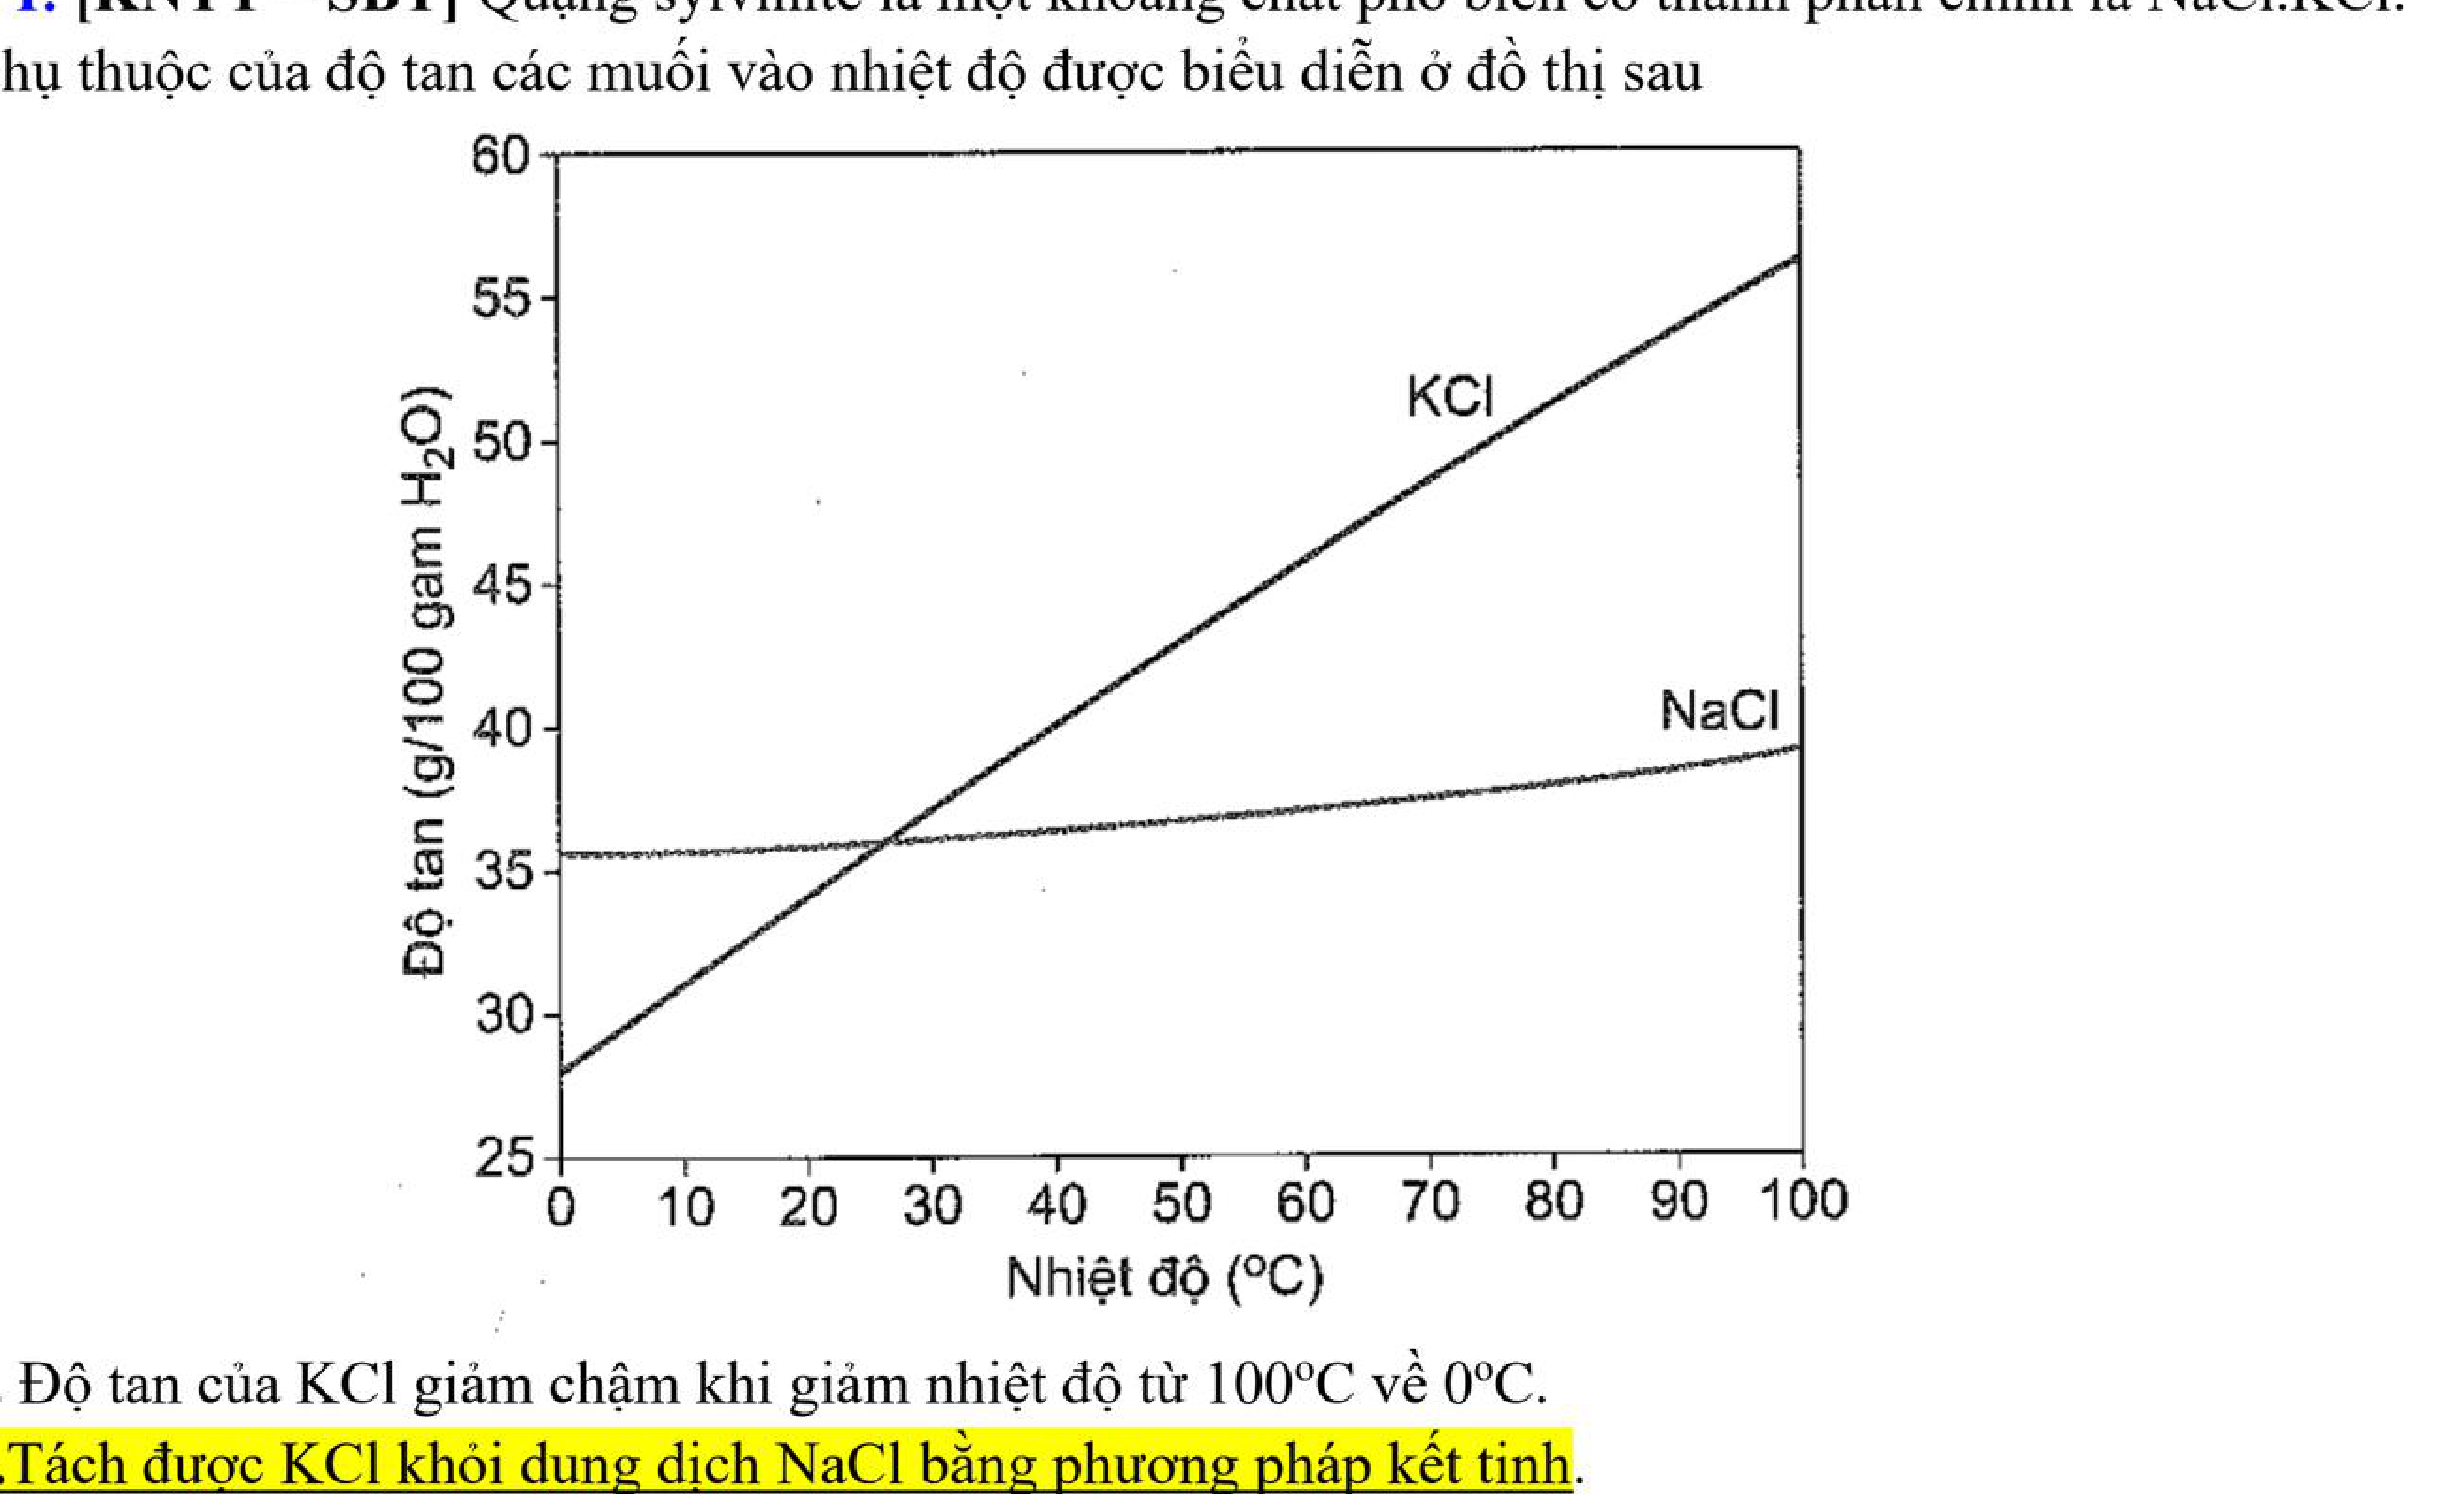
\includegraphics[height=4.6cm]{images_crop_de19/p2_cau1_do_thi_do_tan.png}}\vspace{1pt}
\choiceTF
{Độ tan của \ce{KCl} giảm chậm khi giảm nhiệt độ từ $100^\circ\text{C}$ về $0^\circ\text{C}$.}
{Tách được \ce{KCl} khỏi dung dịch \ce{NaCl} bằng phương pháp kết tinh phân đoạn.}
{Độ tan của \ce{NaCl} tăng nhanh khi nhiệt độ từ $0^\circ\text{C}$ đến $100^\circ\text{C}$.}
{Độ tan của \ce{KCl} giảm nhanh hơn của \ce{NaCl} khi giảm nhiệt độ từ $100^\circ\text{C}$ về $0^\circ\text{C}$.}
\loigiai{}
\end{ex}

\begin{ex}
Mỗi phát biểu sau đây về kim loại kiềm là đúng hay sai?
\choiceTF
{Thứ tự giảm dần tính kim loại của các kim loại kiềm là: Cs, Rb, K, Na, Li.}
{Phương pháp chung để điều chế kim loại kiềm là điện phân dung dịch.}
{Để bảo quản kim loại Na cần ngâm Na trong cồn tinh khiết.}
{\ce{Na2O} tan trong nước tạo dung dịch trong suốt và thoát ra khí \ce{H2}.}
\loigiai{}
\end{ex}

\begin{ex}
Cho các mẫu nước được đánh dấu X, Y, Z, T có chứa các ion theo bảng sau:
\par\vspace{1pt}{\centering
\small\renewcommand{\arraystretch}{0.92}
\begin{tabular}{|c|l|}
\hline
\textbf{Mẫu nước} & \textbf{Các ion chủ yếu có trong mẫu nước} \\
\hline
X & \ce{Ca^2+}, \ce{Mg^2+} (nhiều), \ce{Cl-}, \ce{SO4^2-} \\
Y & \ce{Ca^2+}, \ce{Mg^2+} (nhiều), \ce{HCO3-} \\
Z & \ce{Na+}, \ce{K+}, \ce{HCO3-} \\
T & \ce{Ca^2+}, \ce{Mg^2+} (nhiều), \ce{Cl-}, \ce{SO4^2-}, \ce{HCO3-} \\
\hline
\end{tabular}\par}\vspace{1pt}
\choiceTF
{Nước X và Y đều là nước có tính cứng vĩnh cửu.}
{Có thể loại bỏ tính cứng của nước T bằng cách đun nóng.}
{Có thể loại bỏ tính cứng của nước Y bằng dung dịch \ce{Na2CO3} dư.}
{Có thể phân biệt X, Y, Z và T bằng cách đun nóng nhẹ và dùng dung dịch \ce{NaOH}.}
\loigiai{}
\end{ex}

\begin{ex}
Hợp chất của kim loại calcium có nhiều ứng dụng quan trọng trong thực tiễn đời sống và sản xuất.
\choiceTF
{Hợp chất của calcium được dùng để đúc tượng, bó bột khi gãy xương là thạch cao nung (\ce{CaSO4.H2O}).}
{Vôi sống (\ce{CaO}) được dùng phổ biến để khử chua cho đất trồng trọt.}
{Phương trình hoá học của phản ứng tạo thạch nhũ trong các hang động đá vôi là: $\ce{CaCO3 + CO2 + H2O -> Ca(HCO3)2}$.}
{Thành phần hoá học chính của vỏ các loài ốc, sò, hến là calcium carbonate (\ce{CaCO3}).}
\loigiai{}
\end{ex}

\newpage

\noindent
\textbf{PHẦN III (1,5 điểm -- 6 câu): Câu trắc nghiệm yêu cầu trả lời ngắn.}\\
\textit{Thí sinh trả lời từ câu 1 đến câu 6.}

\setcounter{ex}{0}

\begin{ex}
Cho các kim loại sau: Li, Na, Ca, Mg, Fe, Cu, K, Zn, Ag, Rb. Có bao nhiêu kim loại kiềm trong dãy trên?
\par\noindent\textit{Trả lời:} \dotfill
\loigiai{}
\end{ex}

\begin{ex}
Cho sơ đồ các phản ứng sau theo đúng tỉ lệ mol:\\
(1) $\ce{2X1 + 2X2 -> 2X3 + H2}$\\
(2) $\ce{X3 + CO2 -> X4}$\\
(3) $\ce{X3 + X4 -> X5 + X2}$\\
(4) $\ce{2X6 + 3X5 + 3X2 -> 2Fe(OH)3 + 3CO2 + 6KCl}$\\
Khối lượng mol của chất $\text{X}_5$ là bao nhiêu g/mol?
\par\noindent\textit{Trả lời:} \dotfill
\loigiai{}
\end{ex}

\begin{ex}
Cho các phát biểu sau:\\
(1) Soda là chất bột màu trắng, tan trong nước tạo môi trường trung tính.\\
(2) Soda dùng làm mềm nước cứng.\\
(3) Soda bền với nhiệt hơn so với baking soda.\\
(4) Chất béo bị thuỷ phân trong dung dịch soda tạo thành xà phòng.\\
(5) Có thể dùng baking soda thay cho soda trong việc tẩy rửa lớp dầu, mỡ bám vào bồn cầu.\\
Có bao nhiêu phát biểu đúng trong các phát biểu trên?
\par\noindent\textit{Trả lời:} \dotfill
\loigiai{}
\end{ex}

\begin{ex}
Trong số các chất sau: \ce{Ca(OH)2}, \ce{Na2CO3}, \ce{Na3PO4}, \ce{KCl}, có bao nhiêu chất có thể dùng để làm mềm nước có tính cứng tạm thời?
\par\noindent\textit{Trả lời:} \dotfill
\loigiai{}
\end{ex}

\begin{ex}
Trong công nghiệp, người ta sản xuất xút (\ce{NaOH}) từ muối ăn bằng phương pháp điện phân dung dịch có màng ngăn xốp. Tính khối lượng (tấn) \ce{NaCl} cần dùng để sản xuất 15 tấn \ce{NaOH} với hiệu suất của toàn bộ quá trình là 80\% (kết quả làm tròn đến hàng phần mười).
\par\noindent\textit{Trả lời:} \dotfill
\loigiai{}
\end{ex}

\begin{ex}
Carnallite là muối khoáng kép ngậm nước có công thức dạng $\ce{KCl.MgCl2.nH2O}$. Khi nung nóng 5,55 gam carnallite, thu được 3,39 gam muối khan. Mặt khác, nếu cho 5,55 gam carnallite tác dụng hoàn toàn với dung dịch \ce{NaOH} dư, thu được kết tủa. Lọc và nung kết tủa đến khối lượng không đổi thì khối lượng chất rắn giảm 0,36 gam so với khối lượng kết tủa ban đầu. Xác định giá trị của $n$.
\par\noindent\textit{Trả lời:} \dotfill
\loigiai{}
\end{ex}

\Closesolutionfile{ans}
\end{document}
